\chapter{Distribution Command}
\label{chp:distribution}
\index{distr|(}
Particle distributions can be read in or generated by specifying rms beam quantities.
The allowed parameters are described in Table \ref{tab:distrparam}.

Particle distributions are generated separately in all three phase space planes.
There are limited correlations between planes e.g. between longitudinal and transverse ($r51,r52,r61,r62$).
Besides an efficient parallel Gaussian distribution generator based on a parallelized 
``Method of Rejection'',
a more general algorithm for generating
distributions is available \cite{JohoDist}. The shape of the binomial distribution is governed by
one parameter $m$. By varying this single parameter one obtains the most commonly 
used distributions for our
type of simulations as, listed in Table \ref{tab:binomdist}.

If NBIN is larger than one the distribution is binned in energy and for each bin a separate field solve is
performed when using the electrostatic solvers.
 
\begin{table}[h!]
  \begin{center} \footnotesize
    \caption{Different distributions specified by a single parameter $m$}
    \label{tab:binomdist}
    \begin{tabular}{|l|l|l|l|}
      \hline
      \bf m & \bf Distribution & \bf Density & \bf Profile \\
      \hline
      0.0 & Hollow shell  & $\frac{1}{\pi}\delta(1-r^2)$ &$\frac{1}{\pi}(1-r^2)^{-0.5}$\\
      \hline
      0.5 & Flat profile  & $\frac{1}{2\pi}(1-r^2)^{-0.5}$ & $\frac{1}{2}$\\
      \hline
      1.0 & Uniform  & $\frac{1}{\pi}$ & $\frac{2}{\pi}(1-x^2)^{0.5}$\\
      \hline
      1.5 & Elliptical  & $\frac{3}{2\pi}(1-r^2)^{0.5}$ & $\frac{1}{4}(1-x^2)$ \\
      \hline
      2.0 & Parabolic  & $\frac{2}{\pi}(1-r^2)$ & $\frac{3}{8\pi}(1-x^2)^{1.5}$ \\
      \hline
      $\rightarrow \infty$ & Gaussian  & $\frac{1}{2\pi\sigma_x\sigma_y}exp(-\frac{x^2}{2\sigma_x^2} -\frac{y^2}{2\sigma_y^2})$ & 
      $\frac{1}{\sqrt{2\pi}*\sigma_x}exp(-\frac{x^2}{2\sigma_x^2}) $ \\
      \hline
    \end{tabular}
  \end{center} 
\end{table}
There are also special distribution commands.
\begin{enumerate}
%\item {\it GUNGAUSS} will create a distribution that is uniform in $x$ and $y$ (with the
%radius in each plane given by SIGMAX and SIGMAY) and with a Gaussian distribution longitudinally (given by SIGMAT).
%This distribution is cold in the transverse direction and has a uniform temperature given by the initial kinetic energy in
%eV specified by the PT and the SIGMAPT variables.
%\item {\it GUNGAUSS3D} is identical to {\it GUNGAUSS} except that it generates a distribution that is Gaussian in the
%transverse planes as well.
%\item {\it GUNUNIFORM} is the same as {\it GUNGAUSS} except that the longitudinal distribution is uniform. The result is a
%uniformaly filled cylinder of charge. (SIGMAT gives the length of the cylinder in meters.)
%\item {\it UNITUNIL} will create a 3D spatial Uniform distribution in transverse as well as longitudinal direction, cold
%in transverse direction and with a uniform temperature given by the initial kinetic in eV specified by the PT and the SIGMAPT variables.
\item {\it GUNGAUSSFLATTOPTH} will create a distribution that is uniform
transversely. The longitudinal profile has a
Guassian rise and fall with a flat top distribution in between. More details are
given in Section \ref{sec:dist_flattop}. This distribution has thermal emittance as defined at \ref{sec:them}.

\item {\it ASTRAFLATTOPTH} is the same like {\tt GUNGAUSSFLATTOPTH} except it uses a low noise Hammersley generator in the longitudinal direction.

\end{enumerate}

\begin{table}[h!]
  \begin{center}
    \footnotesize
    \caption{Parameters for the DISTRIBUTION command}
    \begin{tabular}{|l|l|}
      \hline
      Parameter & Purpose \\
      \hline
      \mytabline{DISTRIBUTION}{\texttt{FROMFILE} or \texttt{GAUSS} or \texttt{BINOMINAL}  or \texttt{ROTSYMBINOMIAL}}   
      \mytabline{}{\texttt{GUNGAUSSFLATTOPTH} or \texttt{ASTRAFLATTOPTH}}
      \mytabline{FNAME}{Specifies the filename of a particle distribution to be read in}
      \mytabline{XMULT}{Scales the x coordinate: $x = XMULT*x$}	
      \mytabline{PXMULT}{Scales the px coordinate: $px = PXMULT*px$}
      \mytabline{YMULT}{Scales the y coordinate: $y = YMULT*y$}
      \mytabline{PYMULT}{Scales the py coordinate: $py = PYMULT*py$}
      \mytabline{TMULT}{Scales the t coordinate: $t = TMULT*t$}
      \mytabline{PTMULT}{Scales the pt coordinate: $pt = PTMULT*pt$}
      \hline                        
      \mytabline{$SIGMAX$}{$\rms{x}$ see Chapter on Notation }
      \mytabline{$SIGMAPX$}{$\rms{p}_x$ see Chapter on Notation }
      \mytabline{$SIGMAY$}{$\rms{y}$ see Chapter on Notation }
      \mytabline{$SIGMAPY$}{$\rms{p}_y$ see Chapter on Notation }
      \mytabline{$SIGMAT$}{$\rms{t}$ see Chapter on Notation }
       \mytabline{TRANSVCUTOFF}{Defines the transverse cut-off of \texttt{GUNGAUSS3D} in units of $\sigma$}
      \mytabline{$PT$}{$\langle p_t \rangle$ see Chapter on Notation }
      \mytabline{$SIGMAPT$}{$\rms{p}_t$ see Chapter on Notation }
      \hline
       \mytabline{mx} {Defines the transverse distribution (see Table \ref{tab:binomdist}) }
      \mytabline{my} {Defines the transverse distribution (see Table \ref{tab:binomdist}) }
      \mytabline{mt} {Defines the longitudinal distribution (see Table \ref{tab:binomdist}) }
      \hline
      \mytabline{CORRX} {Defines the $x$, $p_x$ correlation }
      \mytabline{CORRY} {Defines the $y$, $p_y$ correlation }
      \mytabline{CORRT} {Defines the $t$, $p_t$ correlation }
      \hline
    \end{tabular}
  \end{center}
 \end{table}
      
\begin{table}[h!]
  \footnotesize
  \caption{Parameters of the distribution command}
  \label{tab:distrparam}
  \begin{center}
    \begin{tabular}{|l|l|}
      \hline
      Parameter & Purpose \\
      \hline
      \mytabline{TEMISSION} {Defines the length of the emission process [s] }
      \mytabline{NBIN} {How many energy bins begin used }
      \mytabline{DEBIN} {Defines a energy band $dE$ [MeV].}
      \mytabline{} {If the maximal energy difference between all bins are}
      \mytabline{} {smaller than $dE$ all bins are merged into one bin.}
      \hline
      \mytabline{ELASER}{Laser energy (eV)}
      \mytabline{SIGLASER}{Sigma of (uniform) laser spot size (m)}
      \mytabline{W}{Workfunction of material (eV)}
      \mytabline{FE}{Fermi energy (eV)}
      \mytabline{AG}{Acceleration Gradient (MV/m)}
      \hline
    \end{tabular} 
  \end{center}
\end{table}

The following example reads in a distribution from a file and scales the coordinates:
\begin{verbatim}
DistFile:DISTRIBUTION, DISTRIBUTION=FROMFILE,
         FNAME="../Dist/inpdist1finitecur.dat",
         XMULT=0.06816207, YMULT=0.06816207,
         TMULT=1.0*beta*0.06816207,
         PXMULT=1/gambet, PYMULT=1/gambet,
         PTMULT=1.0/beta^2/gamma;
\end{verbatim}

The file with the data has to have the following format:\\
\\
$N$\\
$x_1$ $px_1$ $y_1$ $py_1$ $z_1$ $pz_1$\\
$x_2$ $px_2$ $y_2$ $py_2$ $z_2$ $pz_2$\\
.\\
.\\
$x_N$ $px_N$ $y_N$ $py_N$ $z_N$ $pz_N$,\\
\\
where $N$ is the number of particles, the vector $(x_i,y_i,z_i)$ describes the position of the i-th particle and the vector $(px_i, py_i, pz_i)$ its momentum in as defined in section
\ref{sec:variablesopalt} and section \ref{sec:variablesopalcycl}.

\section{Correlations for Gaussian Distribution (Experimental)}

To generate gaussian initial distribution with dispersion, first we
generate the uncorrelated gaussian inputs matrix $R=(R1,...,R_n)$.
The mean of $R_i$ is $0$ and the standard deviation squared is 1. Then
we correlate $R$.
The correlation coefficient matrix $\sigma$ in $x,p_x,t,p_t$ phase space reads: \\

$ \hspace{0.5cm}x \hspace{0.8cm}  px  \hspace{0.9cm} t\hspace{1.0cm} pt\\$
$\sigma= \left[
\begin{array}{cccc}
1    &c_x&r51    &r61\\
c_x&1    &r52    &r62\\
r51  &r52  &1      &c_t\\
r61  &r62  &c_t  &1\\
\end{array}
\right].$ \\

The Cholesky decomposition of the symmetric positive-definite matrix $\sigma$ is $\sigma=C^TC$, then the correlated distribution is $C^TR$.

\textbf{Note}: This correlation works for the moment only with the gaussian distribution.

\subsection{Example}
Let the initial correlation coefficient matrix be:

$\sigma= \left[
\begin{array}{cccc}
1      &0.756  &0.023    &0.496\\
0.756  &1      &0.385    &-0.042\\
0.023  &0.385  &1        &-0.834\\
0.496  &-0.042 &-0.834   &1\\

\end{array}
\right]$ \\
then the corresponding distribution command read:
\begin{verbatim}
Dist:DISTRIBUTION, DISTRIBUTION=gauss,
     sigmax=4.796e-03, sigmapx=231.0585, corrx=0.756,
     sigmay=23.821e-03, sigmapy=1.6592e+03, corry=-0.999,
     t=0.466e-02, sigmat=0.466e-02, pt=72e6, 
     sigmapt=74.7, corrt=-0.834,
     r61=0.496, r62=-0.042, r51=0.023, r52=0.385;
\end{verbatim}

\section{Thermal Emittance}
\label{sec:them}
The thermal emittance calculation is based on \cite{flo:97, clen:2000} where  $P(E_f,E_{ph}=\hbar\omega)$ the probability for a photon of energy $E_{ph}$ exiting an electron to a final state energy $E_f$ is

\begin{equation} P(E_f,E_{ph}=\hbar\omega) \propto N_f(E_f) N_i(E_f - E_{ph}=\hbar\omega) \text{ with}\end{equation}


 $N_f(E_f)$ is the density of final state
and $N_i(E_f - E_{ph})$ is the density of initial state.

Two cases, no-scattering (non-equilibrum) and scattering (equilibrium, e-e and e-phonon collisions) can be distinguished. In \opal the non-equilibrum case is considered and a uniform radial distribution is assumed hence: $x_{rms} = \frac{r}{2}$ \footnote{Soon we can generate distributions form virtual cathode images}.

Photoemission from a metal involves fist the absorption of a photon with:
\begin{equation} 
\hbar\omega > \Phi_e
\end{equation}
where $\Phi_e = \Phi - \Delta$ is the reduced work function.
The reduction is a function of the applied electric field $E_c$:
\begin{equation}
\Delta = e \sqrt{e E_c / 4 \pi \epsilon_0}.
\end{equation}

Electrons are emitted isotropic into the half-sphere with: $E_{kin} = \eps_{f} + \hbar\omega$.

Particles with angel $\varphi$ larger than $\varphi_{max}=\arccos{\sqrt{(\eps_f + \Phi_e / E_{kin})}}$ will pass the potential barrier. 
\begin{equation} p_x = p \sin{\varphi} \cos{\theta},~ \varphi=[0\dots \varphi_{max}],~  \theta=[0\dots \pi] \end{equation}
and 
\begin{equation} p= m_0 c \sqrt{\gamma^2 - 1}. \end{equation}

The following parameters defines the thermal emittance:  $r_{rms}$, material such as Cu, Fe, Cs2Te $\rightarrow \Phi, \eps_f$, 
the laser energy given by $\hbar\omega$ and the electric field $E_c$ which enters in the Schottky effect calculation.

This is a example of an \opal distribution definition with thermal emittance similar to the example in \cite{clen:2000} p.199.

\begin{verbatim}
Dist1:DISTRIBUTION, DISTRIBUTION = GUNGAUSSFLATTOPTH,
      sigmax=0.00054, sigmapx=0.0, corrx=0.0,
      sigmay=0.00054, sigmapy=0.0, corry=0.0,
      sigmat=lzFlatTop, pt=1.0, sigmapt=0.0, corrt=0.0,
      sigmarise=0.5e-12, sigmafall=0.5e-12, 
      flattoptime=10e-12, cutoffrise=3.0, cutofffall=3.0,
      TEMISSION=TEmis, NBIN=50, DEBIN=80,
      ELASER=4.6, SIGLASER=0.001, W=4.6, FE=7.0, AG=84;  

\end{verbatim}

\section{Flattop Distribution}
\label{sec:dist_flattop}.

\begin{figure}[h]
  \begin{center}
    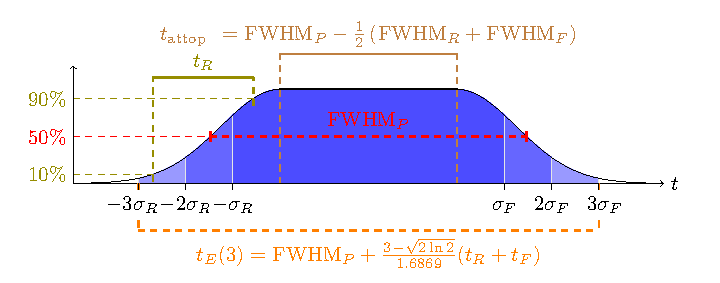
\includegraphics[width=0.8\textwidth]{./figures/flattop.pdf}
    \caption{\textsc{OPAL} Gauss-Flattop-Distribution}
    \label{fig:flattop}
  \end{center} 
\end{figure}

Figure \ref{fig:flattop} depicts parameters needed to specify a Gauss-Flattop
distribution in \textsc{OPAL} where $c$ stands for cutoff, $P$ for pulse, $R$
for rise and $F$ for fall. A Gauss-Flattop distribution is defined as half a
Gauss plus a uniform (flat-top) part plus half a Gauss with the parameters
$\sigma_R$, $\sigma_F$ and $t_\mathrm{flattop}$. For practical reasons we
replace these three parameters with the following measurable parameters
\[ 
    t_R = \left(\sqrt{2\ln{\left(10\right)}}-\sqrt{2\ln{\left(\frac{10}{9}\right)}}\right)\sigma_R = 1.6869\sigma_R, \;\; t_F = 1.6869\sigma_F \;\; \mathrm{and}
\]
\[
    \mathrm{FWHM}_P = t_\mathrm{flattop} + \sqrt{2\ln{2}}(\sigma_R+\sigma_L)\mathrm{.}
\]
%    
The emission time ($t_E$) with a given cutoff $c$ in terms of input parameters
is given by
%
\begin{eqnarray*}
    t_E(c) &=& \mathrm{FWHM}_{P} - \frac{1}{2} \mathrm{FWHM}_R - \frac{1}{2}
    \mathrm{FWHM}_F + c\sigma_R + c\sigma_F \\
    &=& \mathrm{FWHM}_{P} + \frac{c - \sqrt{2\ln{2}}}{1.6869} (t_R + t_F) \mathrm{.}
\end{eqnarray*}
%
In \textsc{OPAL} this distribution can be specified by the following
distribution command (thermal emittance enabled)
%
\begin{verbatim}
Dist1:DISTRIBUTION, DISTRIBUTION = "GUNGAUSSFLATTOPTH",
    sigmax = 0.000275 * 2., sigmapx = 0.0, corrx = 0.0,
    sigmay = 0.000275 * 2., sigmapy = 0.0, corry = 0.0,
    sigmat = 0.0, pt = 0.0, sigmapt = 0.0, corrt = 0.0,
    tRise = 0.7e-12, tFall = 0.7e-12, tPulseFWHM = 9.9e-12,
    ekin = 0.63, NBIN = 50, DEBIN = 80;
\end{verbatim}
%
where \texttt{tRise} ($t_R$, olive in Figure 1), \texttt{tFall} and
\texttt{tPulseFWHM} ($\mathrm{FWHM}_P$, red in Figure 1) in seconds $[s]$ define
the shape of the Gauss-Flattop distribution. The default cutoff is \texttt{3.0}.
This can be changed by adding e.g. \texttt{cutoff = 4.0} to the distribution
command.

\subsection{Legacy Mode}

We provide a legacy mode for flattop distribution. The following
old input specification
%
\begin{verbatim}
SRise = 0.7e-12;
SFall = 0.7e-12;
CRise = 3.0;
CFall = 3.0;
TFlatTop = 9.9e-12*0.925;
TEmis = TFlatTop + CRise* SRise + CFall* SFall;

value,{TFlatTop,TEmis};

Dist1:DISTRIBUTION, DISTRIBUTION = "GUNGAUSSFLATTOPTH",
    sigmax = 0.000270*2.0, sigmapx = 0.0, corrx = 0.0,
    sigmay = 0.000270*2.0, sigmapy = 0.0, corry = 0.0,
    sigmat = 0.0, pt = 0.0, sigmapt = 0.0, corrt = 0.0, ekin = 0.4,
    sigmarise = 0.7e-12, sigmafall = 0.7e-12, flattoptime = 9.9e-12*0.925,
    cutoffrise = CRise, cutofffall = CFall,
    TEMISSION = TEmis, NBIN = 10, DEBIN = 80;
\end{verbatim}
%
can be replaced by
%
\begin{verbatim}
st1:DISTRIBUTION, DISTRIBUTION = "GUNGAUSSFLATTOPTH",
    sigmax = 0.000275 * 2., sigmapx = 0.0, corrx = 0.0,
    sigmay = 0.000275 * 2., sigmapy = 0.0, corry = 0.0,
    sigmat = 0.0, pt = 0.0, sigmapt = 0.0, corrt = 0.0, ekin = 0.4,
    tRise = 0.7e-12, tFall = 0.7e-12, tPulseFWHM = 9.9e-12*0.925,
    NBIN = 10, DEBIN = 80, LEGACYMODE=TRUE;
\end{verbatim}
%
and should produce the same results. Make sure to enable the \texttt{LEGACYMODE}
option to create the flattop distribution in legacy mode! 

\index{distr|)}



